\chapter{実装}
\label{chap:poordirection}

\section{システムの流れ}

\section{iOSアプリケーション}
iOSアプリケーションを作成するにあたり, 以下の言語とライブラリ, 統合開発環境を利用した.(表3.1参照.)

\begin{table}
\begin{center}
\begin{tabular}{|l|l|} \hline
Xcode &  \\ \hline
Objective-C 2.0 & \\ \hline
Tesseract-OCR & \\ \hline
OpenCV & \\ \hline
\end{tabular}
\end{center}
\caption{iOSアプリケーション作成時に利用した環境のバージョン一覧}
\end{table}

\subsection{ユースケース}
iOSアプリケーションは, 画像から取得した文字列をWebアプリケーションのデータベースに送信することを目的としている.

ユーザがiOSデバイスのカメラを用いて撮影した画像から, 文字列を検出する.
その文字列をWebアプリケーションのデータベースに送信し, 集積する.
\begin{figure}
\begin{center}
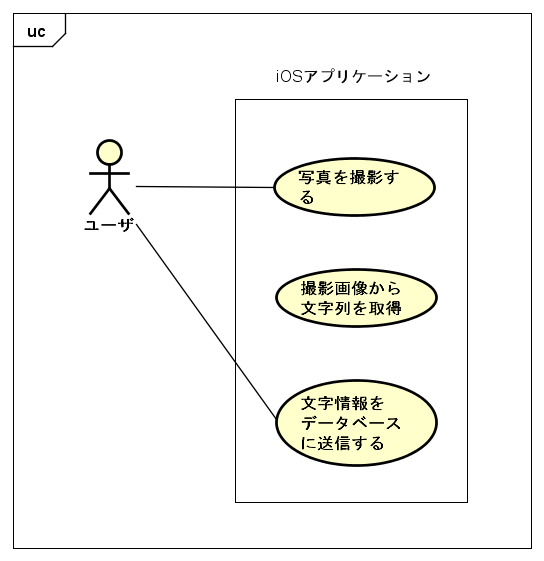
\includegraphics[width=14cm]{fig/usecase_ios.png}
\end{center}
\caption{iOSアプリケーションのユースケース図}
\end{figure}

\subsection{クラス}
\begin{figure}
\begin{center}
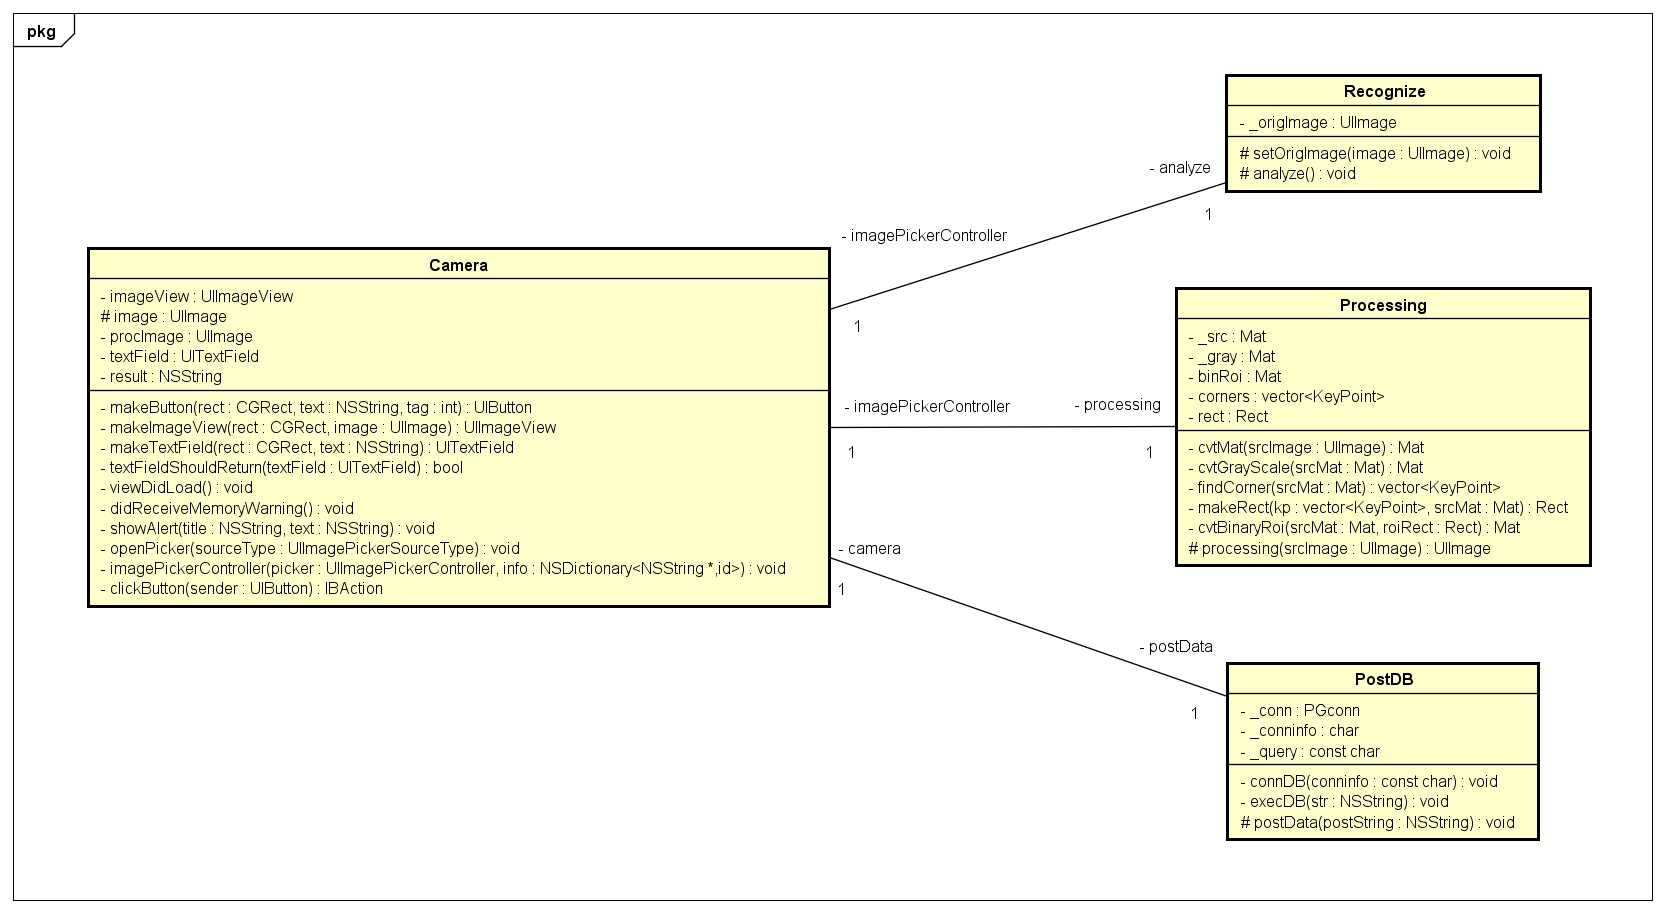
\includegraphics[width=17cm]{fig/class_ios.png}
\end{center}
\caption{iOSアプリケーションのクラス図}
\end{figure}

\subsubsection{3.2.2.1 Cameraクラス}
\begin{itemize}
\item 属性

\begin{itemize}
\item imageView:UIImageView

撮影した画像を出力するためのローカル変数.
出力画像のサイズ等を決定する.

\item image:UIImage

撮影した画像を格納するための変数.

\item procImage:UIImage

Processingクラスにて画像処理された画像を格納するための変数.
procImageに格納されている画像を用いて, 光学的文字認識を行う.

\item textField:UITextField

Recognizeにて取得した文字列を表示するテキストボックス.

\item result:NSString

Recognizeにて取得してきた文字列を格納するためのローカル変数.
\end{itemize}

\item 操作

\begin{itemize}
\item makeButton:UIButton

iOSアプリケーションのMainViewにボタンを作成するメソッド.

ボタンを配置する座標, サイズ, ボタンに書かれる文字列, ボタンに付加するタグを指定して呼び出すことで, iOSアプリケーションのMainViewにボタンを作成し配置する.

\begin{itemize}
\item rect:CGRect

ボタンの座標, サイズを決定する変数.

\item text:NSString

ボタンに書かれる文字列を決定する変数.

\item tag:int

ボタンに整数型のタグを付加するための変数.
\end{itemize}

\item makeImageView:UIImageView

iOSアプリケーションのMainViewに画像を表示するためのSubViewを作成するメソッド.

画像を配置する座標, サイズ, 出力する画像を指定して呼び出すことで, iOSアプリケーションのMainViewに画像を出力する.

\begin{itemize}
\item rect:CGRect

画像を出力するSubViewの座標, サイズを指定する変数.

\item image:UIImage

SubViewに出力する画像を指定する変数.
\end{itemize}

\item makeTextField:UITextField

iOSアプリケーションのMainViewにテキストフィールドを作成するメソッド.

テキストフィールドを配置する座標, サイズ, 入力されるテキストを指定して呼び出すことで, iOSアプリケーションのMainViewにテキストフィールドを作成し配置する.

\begin{itemize}
\item rect:CGRect

テキストフィールドを配置する座標, サイズを指定する変数.

\item text:NSString

テキストフィールドに入力する文字列を指定する変数.
\end{itemize}

\item textFieldShouldReturn:BOOL

テキストフィールドにて, キーボードでリターンキーを押した際の挙動を制御するメソッド.

文字列を編集後にリターンキーを押した際に呼び出され, SubViewとして呼びだされているキーボードを引っ込める.

\begin{itemize}
\item textField:UITextField

編集したい文字列が入力されているテキストフィールド.
\end{itemize}

\item viewDidLoad:void

アプリケーションが起動した際に一度だけ読み込まれるメソッド.

変数の初期化やMainViewにボタン等を配置する際に利用する.

\item didReceiveMemoryWarning:void

iOSアプリケーション使用時に, メモリが不足する際に呼び出されるメソッド.

すべてのViewに対して参照を開放する際に利用する.

\item showAlert:void

アラートビューを表示するメソッド.

アラートビューのタイトルと表示するアラートの内容を指定して呼び出すことで, iOSアプリケーションのMainView上にSubViewとしてアラートが表示される.

\begin{itemize}
\item title:NSString

アラートビューのタイトルを指定する変数.

\item text:NSString

アラートビューに表示するテキストを指定する変数.
\end{itemize}

\item openPicker:void

iOSアプリケーションにて, 画像を取得するためのメソッド.

カメラ, フォトアルバム, フォトライブラリから画像を取得する.

このメソッドでは, iOSのカメラ機能にて撮影した画像を取得する際に呼び出す.

\begin{itemize}
\item sourceType:UIImagePickerSourceType

イメージピッカーの属性を決定する変数.
カメラ, フォトアルバム, フォトライブラリのいずれかから選択する.
\end{itemize}

\item imagePickerController:void

画像取得後に呼び出されるメソッド.

画像を取得した後の処理を行う他クラスのメソッドを呼び出す.

\begin{itemize}
\item picker:UIImagePickerController

画像取得元のイメージピッカーを指定する変数.

\item info:NSDictionary$<$NSString *, id$>$

取得した画像の情報を格納する変数.
\end{itemize}

\item clickButton:IBAction

iOSアプリケーション上のMainViewに配置されているボタンを押下した際に呼び出されるメソッド.

\begin{itemize}
\item sender:UIButton

どのボタンが押下されたのかを決定する変数.
\end{itemize}

\end{itemize}

\end{itemize}

\subsubsection{3.2.2.2 Processingクラス}
\begin{itemize}
\item 属性

\begin{itemize}
\item \_src:Mat

入力画像を指定する変数.

\item \_gray:Mat

グレースケール変換された画像を格納する変数.

\item binRoi:Mat

バイナリスケール変換された画像を格納する変数.

\item corners:vector$<$KeyPoint$>$

検出した特徴点を格納する変数.

\item rect:Rect

特徴点を内包した矩形の座標, サイズ決定する変数.

\end{itemize}

\item 操作

\begin{itemize}
\item cvtMat:Mat

UIImage型の画像をMat型に変換するメソッド.

UIImage型の入力画像を指定して呼び出すことで, OpenCVで処理可能なMat型に変換する.

\begin{itemize}
\item srcImage:UIImage

UIImage型の画像を格納する変数.
\end{itemize}

\item cvtGrayScale:Mat

Mat型画像をグレースケール化するメソッド.

cvtMatにてMat型に変換した入力画像にグレースケール化処理を施す.

\begin{itemize}
\item srcMat:Mat

3チャネルの入力カラー画像を格納する変数.
\end{itemize}

\item findCorner:vector$<$KeyPoint$>$

グレースケール画像から特徴点を検出するメソッド.

cvtGrayScaleにてグレースケール処理を施した画像を指定することで, その画像中から特徴点を検出する.

\begin{itemize}
\item srcMat:Mat

グレースケール画像を格納する変数.
\end{itemize}

\item makeRect:Rect

特徴点を内包する矩形の座標, サイズを決定するメソッド.

特徴点の集合を指定することで, 特徴点の多い部分に注目するための矩形を設定する.

\begin{itemize}
\item kp:vector$<$KeyPoint$>$

特徴点の集合を格納する変数.

\item srcMat:Mat

グレースケール画像を格納するための変数.
\end{itemize}

\item cvtBinaryRoi:Mat

Mat型カラー画像をバイナリ画像へ変換するメソッド.

makeRectにて設定した矩形を指定することで, 注目している範囲をバイナリ画像化する.

\begin{itemize}
\item srcMat:Mat

3チャネルの入力カラー画像を格納する変数.

\item roiRect:Rect

注目する矩形範囲を決定する変数.
\end{itemize}

\item processing

Processingクラスのメソッドをコントロールするメソッド.

\begin{itemize}
\item srcImage:UIImage

CameraクラスのopenPickerControllerメソッドにて取得した撮影画像を格納する変数.
\end{itemize}

\end{itemize}

\end{itemize}

\subsubsection{3.2.2.4 Recognizeクラス}
\begin{itemize}
\item 属性

\begin{itemize}
\item \_origImage:UIImage

光学的文字認識を実行する画像を格納するための変数.
\end{itemize}

\item 操作

\begin{itemize}
\item setOrigImage:void

光学的文字認識を実行する画像を取得するためのメソッド.

Processingクラスのprocessingメソッドにて処理の施された画像を受け取り, \_origImageに格納する.
\begin{itemize}
\item image:UIImage

光学的文字認識を施す画像を指定する変数.
\end{itemize}

\item analyze:void

Tesseract-OCRによる光学的文字認識を実行するメソッド.
\end{itemize}

\end{itemize}

\subsubsection{3.2.2.3 PostDBクラス}
\begin{itemize}
\item 属性

\begin{itemize}
\item \_conn:PGconn

PostgreSQLデータベースとの接続状態を格納する構造体.

\item \_conninfo:const char

PostgreSQLデータベースの接続する際に必要となる情報を格納する変数.

\item \_query:char

接続したPostgreSQLにて実行するクエリを決定する変数.
\end{itemize}

\item 操作

\begin{itemize}
\item connDB:void

WebアプリケーションのPostgreSQLに接続するメソッド.
\begin{itemize}
\item conninfo:const char

PostgreSQLへの接続状態を保存する変数.
\end{itemize}

\item execDB:void

WebアプリケーションのPostgreSQLデータベースへクエリを発行し, データベースへデータを追加する.
\begin{itemize}
\item str:NSString

PostgreSQLデータベースへ送信する文字列を決定する変数.
\end{itemize}

\item postData:void

PostDBクラスのメソッドをコントロールするメソッド.
\begin{itemize}
\item postString:NSString

WebアプリケーションのPostgreSQLデータベースへ送信する文字列を決定する変数.
\end{itemize}

\end{itemize}

\end{itemize}

\section{Webアプリケーション}
Webアプリケーションを作成するにあたり, 以下の言語とライブラリ, サービスを利用した.(表3.2参照.)

\begin{table}
\begin{center}
\begin{tabular}{|l|l|} \hline
Ruby on Rails & \\ \hline
PostgreSQL & \\ \hline
Heroku & \\ \hline
\end{tabular}
\end{center}
\caption{Webアプリケーション作成時に利用した環境のバージョン一覧}
\end{table}

\subsection{ユースケース}
Webアプリケーションは, iOSアプリケーションにて集積したデータ(画像から取得した文字列, データをデータベースにPOSTした日付)を閲覧, 検索することを目的とする.

iOSアプリケーションから送信された全データを閲覧することができ, 文字列, 送信した日付で検索することができる.
\begin{figure}
\begin{center}
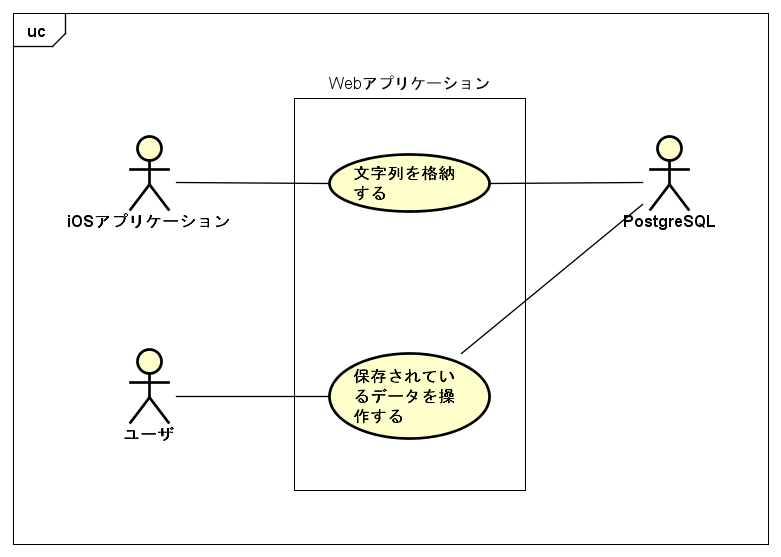
\includegraphics[width=14cm]{fig/usecase_web.png}
\end{center}
\caption{Webアプリケーションのユースケース図}
\end{figure}

\subsection{クラス}
\subsubsection{3.3.2.1Userクラス}
\begin{itemize}
\item 属性

\begin{itemize}
\item current\_sign\_in\_at:datetime

Webアプリケーションにユーザ登録したユーザがサインインした時刻を記録するカラム.

\item current\_sign\_in\_ip:datetime

ユーザがサインインした際のリモートIPを記録するカラム.

\item email:string

ユーザのサインイン時に利用するEメールアドレスを記録するカラム.

\item last\_sign\_in\_at:datetime

ユーザが最終サインインした時刻を記録するカラム.

\item last\_sign\_in\_ip:datetime

ユーザが最終サインインした際のリモートIPを記録するカラム.

\item remenber\_created\_at:datetime

ユーザ登録した時刻を記録するカラム.

\item reset\_password\_sent\_at:datetime

パスワードをリセットする操作を行った際の時刻を記録するカラム.

\item reset\_password\_token:string

パスワードをリセットする操作を行った際に設定した新しいパスワードを記録するカラム.

\item sign\_in\_count:int

ユーザがサインインした回数を記録するカラム.
\end{itemize}

\end{itemize}

\subsubsection{3.3.2.2 StringDBクラス}
\begin{itemize}
\item 属性

\begin{itemize}
\item string:string

光学的文字認識にて取得した文字列を記録するカラム.
\end{itemize}

\end{itemize}

\begin{figure}
\begin{center}
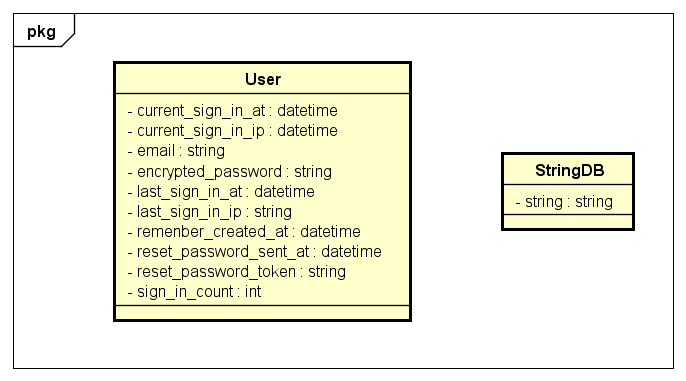
\includegraphics[width=17cm]{fig/class_web.png}
\end{center}
\caption{Webアプリケーションのクラス図}
\end{figure}

%\section{VPSサーバ}
%\subsection{環境構築}
